\documentclass[10pt, compress]{beamer}

% \usetheme{m}
\usepackage[normalem]{ulem}
\usepackage{booktabs}
\usepackage[scale=2]{ccicons}
\usepackage{minted}

\usepackage{tikz}
% \def\checkmark{\tikz\fill[scale=0.4](0,.35) -- (.25,0) -- (1,.7) -- (.25,.15) -- cycle;} 
\usepackage{amssymb}% http://ctan.org/pkg/amssymb
\usepackage{pifont}% http://ctan.org/pkg/pifont
\newcommand{\cmark}{\ding{51}}%
\newcommand{\xmark}{\ding{55}}%
\usepackage{mwe}

\usemintedstyle{trac}

\newcommand{\Sara}[1]{{\color{blue} Sara: #1}}

\title{Joint Causal Inference (JCI) and protein signalling networks}
\subtitle{Applying the JCI framework to real-world data}
\date{\today}
\author{Alex Khawalid\\\textbf{Supervisor:} Sara Magliacane}
\institute{Universiteit van Amsterdam}

\begin{document}

\maketitle

% Present your project. Address the following issues:
% Theoretical foundation and research question
% Research method and approach taken
% Results and evaluation
% Conclusion, discussion, and future work
% The main difference with the project proposal and the midterm progress presentations, is the focus on the completed project, addressing the research objectives, the theoretical foundation and the results obtained.
% Each presentation may take 15 minutes at most (app. 7 to 8 slides), including 2 minutes for questions.
% Upload your presentation (PDF preferred) on Wednesday June 28nd, before 14.00 hours, in order for the presentations to be downloaded by the course coordinators to a USB stick and have the presentations ready on the central computer in the lecture room. Don't miss the deadline!

\begin{frame}
    \frametitle{Introduction}
    % \textbf{Preliminary knowledge to understand the problem}
    \begin{itemize}
        \item \textit{Causal Discovery:} \begin{itemize}
            \item a field in statistics
            \item aims to uncover causal relations
        \end{itemize}
        \item \textit{Causal relations:}\begin{itemize}
            \item given an intervention that changes a variable X, if a variable Y changes then X causes Y
            \item can be represented by causal graphs
        \end{itemize}
        \item \textit{Joint Causal Inference (JCI):} \begin{itemize}
            \item a framework to do causal discovery over multiple datasets
            \item requires specific algorithms because of deterministic relations
            \item do not scale well, can only handle 6 variables % not sufficient for real datasets
        \end{itemize}
        \item Non-deterministic JCI \begin{itemize}
            \item simplified version, no deterministic relations
            \item no implementation yet
            \item expected to scale better, so can be applied to real world data
        \end{itemize}
    \end{itemize}
\end{frame}

% \begin{frame}{What is Non-deterministic JCI?} 
    
%   \begin{figure}
%     \centering
%     \includegraphics[width=\textwidth]{assignment4_cmap.png}
%     \caption{An overview of how JCI fits into the bigger picture}
%   \end{figure}
% \end{frame}

\section{Research question}
\begin{frame}
    \frametitle{Research question}
    \begin{itemize}
        \item \textbf{Main goal of thesis:}
            \begin{itemize}[<+- | alert@+>]
                \item How does JCI perform on a real-world dataset,  e.g. protein signaling network? 
            \end{itemize}
    
        \item\textbf{The problem:}
            \begin{itemize}[<+- | alert@+>]
                \item JCI cannot scale to the required number of variables
            \end{itemize}
    
        \item\textbf{Solution:}
            \begin{itemize}[<+- | alert@+>]
                \item Implement an algorithm for non-deterministic JCI
                \item Add intervention variables that are not deterministically related to the data 
            \end{itemize}
    \end{itemize}
\end{frame}

% gfci vs fges
% gfci constraint
% fges score-based, pattern of graphs with small balls instead of arrows

\section{Approach}
\begin{frame}
    \frametitle{Approach}
    \textbf{How can we implement non-deterministic JCI?}
    \medskip
    
    \begin{itemize}
        \item Add \emph{intervention variables} representing different perturbations in different datasets 
        \item Remove the intervention variables that are \emph{determined} by other intervention variables
        %\item Remove deterministic relations
        \item Add \emph{background knowledge}, e.g. forbidden edges from system variables to intervention variables
        \item Apply a standard causal discovery algorithm, e.g. GFCI or FGES, to the resulting problem
    \end{itemize}
    
      \bigskip
       \textbf{How can we evaluate our approach?}
  \medskip
  
    \begin{itemize}
        %\item Test on real-world data
        \item Evaluate accuracy with ROC curves for simulated data
        \item Compare results real-world data with other algorithms
    \end{itemize}
\end{frame}


\section{Results}
\begin{frame}
    \frametitle{Results: Simulated Data}
    \begin{figure}
        \centering
        \begin{minipage}{0.6\textwidth}
            \centering
            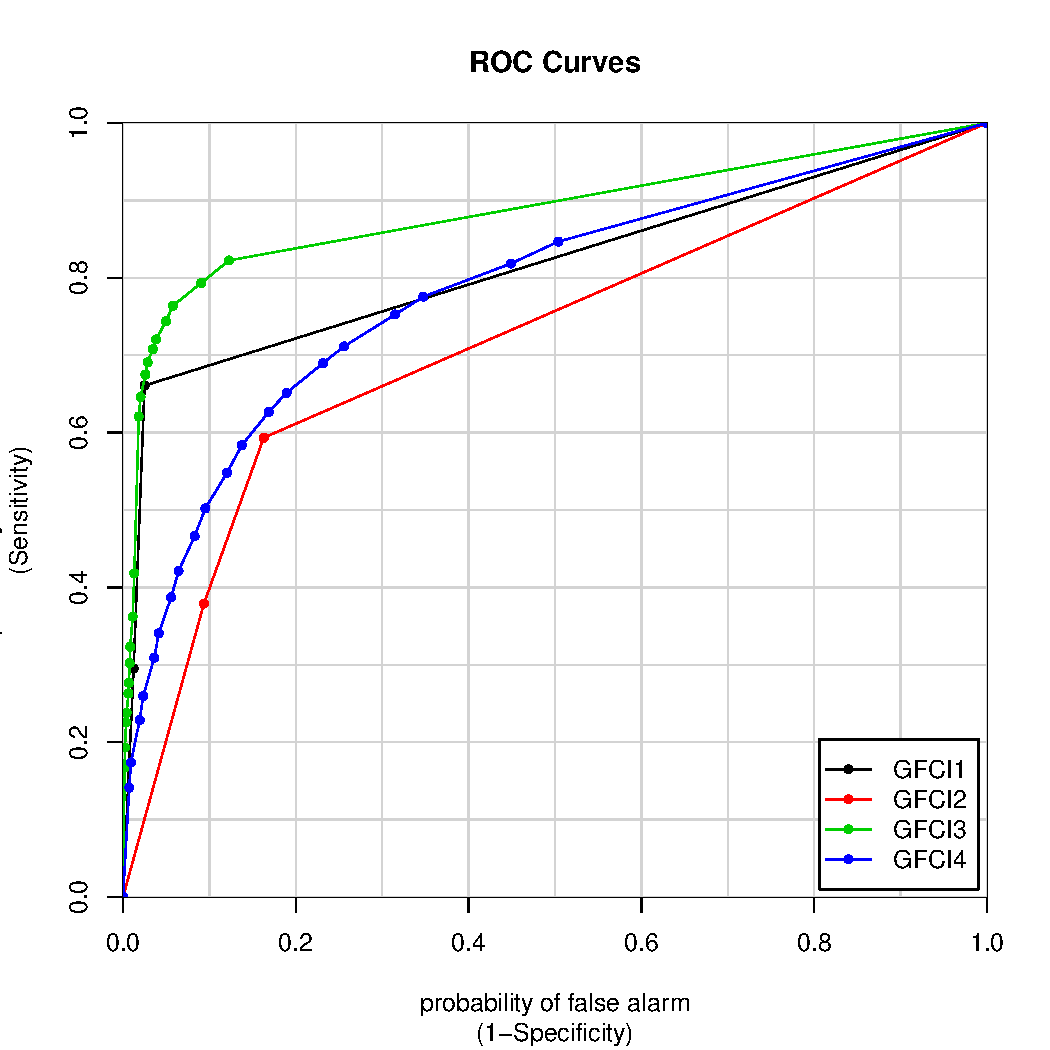
\includegraphics[width=\textwidth]{combinedSimCurvesGFCI}%
        \end{minipage}\hfill
        \begin{minipage}{0.4\textwidth}
            \centering
            \renewcommand{\arraystretch}{1}
            \setlength{\tabcolsep}{5pt}
            \begin{tabular}{|c|c|c|}
                \multicolumn{3}{c}{\large{\textbf{Legend}}}\\
                \hline
                       & Prior & Bootstrapping\\\
                 GFCI1 & \cmark & \xmark\\
                 GFCI2 & \xmark & \xmark\\
                 GFCI3 & \cmark & \cmark \\
                 GFCI4 & \xmark & \cmark\\
                 \hline
            \end{tabular}
        \end{minipage}
    \end{figure}
    % \Sara{Nice! Looks very good. Maybe add a legend or something that explains the difference between the different GFCIs also in the slide. }
    % add sachs graph
    % add gfci graph
\end{frame}


\begin{frame}
    \frametitle{Results: Simulated data}
    \begin{figure}
        \centering
        \begin{minipage}{0.6\textwidth}
            \centering
            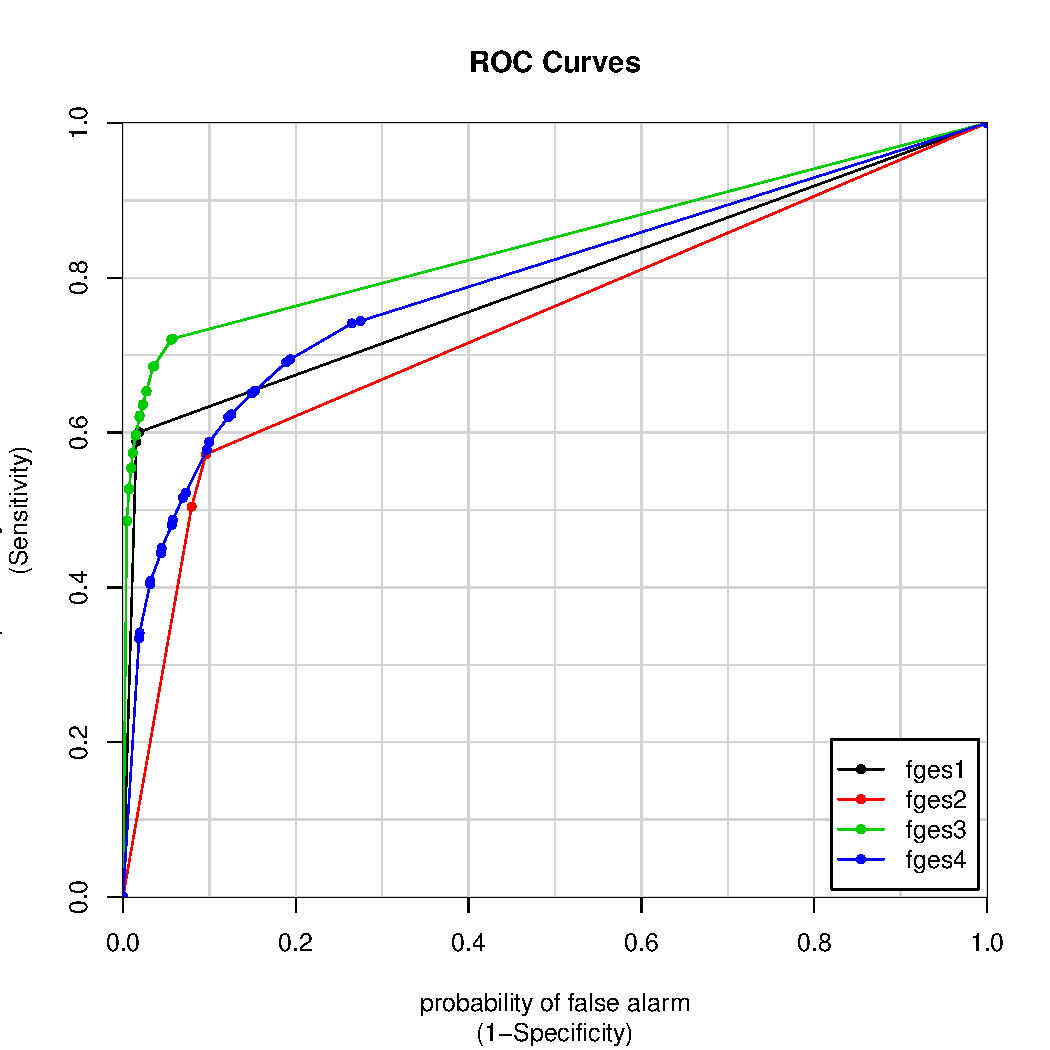
\includegraphics[width=\textwidth]{combinedSimCurvesfges}%
        \end{minipage}\hfill
        \begin{minipage}{0.4\textwidth}
            \centering
            \renewcommand{\arraystretch}{1}
            \setlength{\tabcolsep}{5pt}
            \begin{tabular}{|c|c|c|}
                \multicolumn{3}{c}{\large{\textbf{Legend}}}\\
                \hline
                       & Prior & Bootstrapping\\\
                 FGES1 & \cmark & \xmark\\
                 FGES2 & \xmark & \xmark\\
                 FGES3 & \cmark & \cmark \\
                 FGES4 & \xmark & \cmark\\
                 \hline
            \end{tabular}
        \end{minipage}
    \end{figure}
    
    % add sachs graph
    % add gfci graph
\end{frame}


\begin{frame}
    \frametitle{Results: Sachs dataset}
    \center
    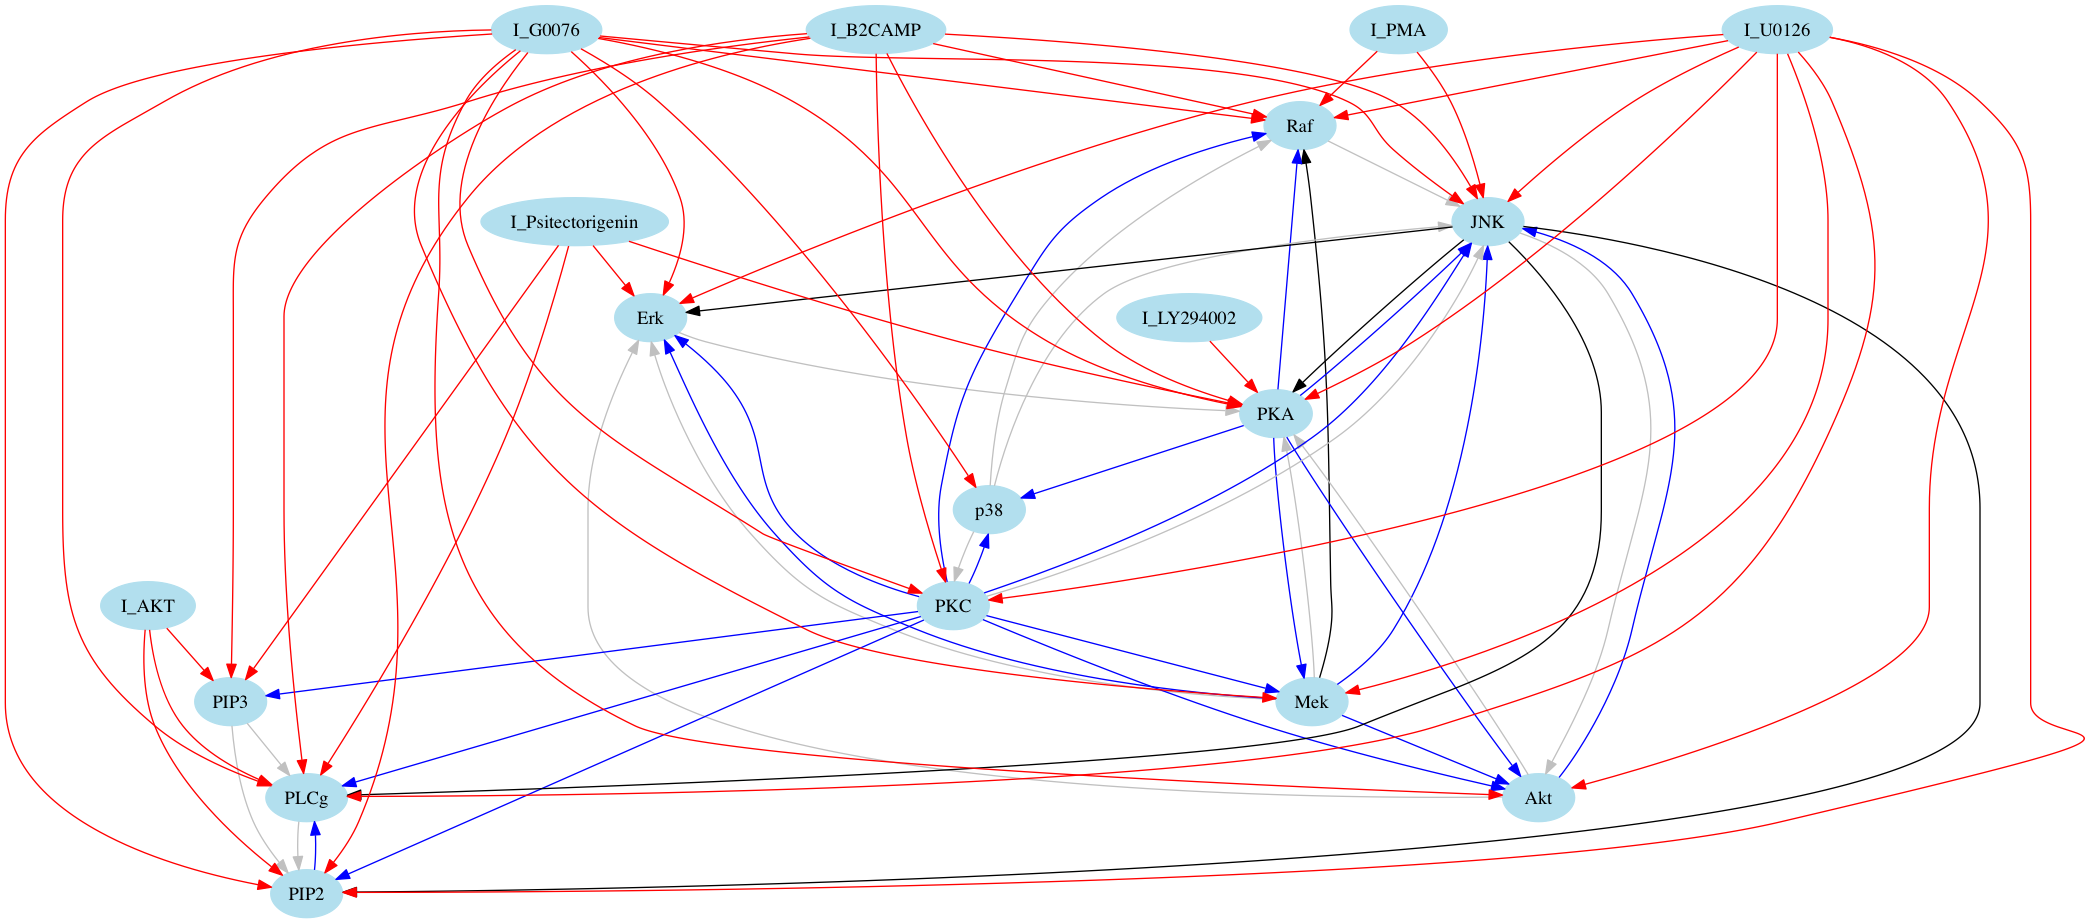
\includegraphics[width=\textwidth]{sachsGraph_bootstrap0_priorTRUEgfciANCSETRAL}
    
    % \Sara{Maybe better the version with the ancestral relations? This is a PAG, and I'm not sure you want to explain what the circles mean...}
    % add sachs graph
    % add gfci graph
\end{frame}


\section{Conclusion}
\begin{frame}
    \frametitle{Conclusion}
    \begin{itemize}
        \item Simplified version of JCI implemented % so now it can scale to real world variables and can is not limited in the methods it can be applied to
        \item Improves results of simulated data compared to other methods only using observational dataset % more than only observational / no numbers
        \item Scalable to real-world data
    \end{itemize}
\end{frame}

\begin{frame}
    \frametitle{Future Work}
    \begin{itemize}
        \item Add more detailed background knowledge % might help with bootstrapping -> more statistical power
        \item Have protein signalling system experts evaluate results
        \item Improve on the scalability of ``deterministic'' JCI by finding a way to combine graphs it produces
    \end{itemize}
\end{frame}

% detailed background: no hidden variables that cause both intervention variables and system variables


\section{Questions}
\begin{frame}{}
\begin{center}
\Huge \textbf{Questions?}
\end{center}
\end{frame}

\end{document}
